\begin{frame}{Bayesian Additive Regression Trees (BART)}

BART is related to both approaches seen before: \pause 
\begin{itemize}
    \item Each tree is constructed in a random manner. \pause 

    \item Each tree tries to capture signal not yet accounted for by the current model. \pause 

    \item The main novelty in BART is the way in which new trees are generated. \pause 
\end{itemize}


But first, some notation: \pause 

\begin{itemize}
    \item Let $K$ denote the number of regression trees. \pause 

    \item $B$ is the number of iterations for which the BART algorithm will be run. \pause 

    \item $\hat{f}_k^b(x)$ is the prediction at $x$ for the $k$th regression tree used in the $b$th iteration. \pause 

    \item At the end of each iteration, all the $K$ trees from $b$ will be summed, 

    \begin{equation*}
        \hat{f}^b(x) = \sum_{k=1}^K \hat{f}_k^b(x) \text{ for } b= 1, \ctods , B. 
    \end{equation*}
\end{itemize}

    
\end{frame}

\begin{frame}{Bayesian Additive Regression Trees (BART)}
    The algorithm is described as follows, \pause 

    \begin{enumerate}
        \item Initialized all trees to have a single root node, with a prediction given by, \pause 

        \begin{equation*}
            \hat{f}_k^1(x) = \frac{1}{nK} \sum_{i=1}^n y_i.
        \end{equation*} \pause 

        \item Compute the prediction in for all the $K$ trees as,  \pause 

        \begin{equation*}
            \hat{f}^1(x) = \frac{1}{n} \sum_{i=1}^n y_i.
        \end{equation*} \pause 

        \item Update each of the $K$ trees in each iteration. \\ \pause 
        For $b = 2, \cdots, B:$  \pause 
        \begin{enumerate}[a]
            \item For $k = 1, \cdots , K$: compute the \textbf{current partial residual}, \pause 
            \begin{equation*}
                r_i = y_i - \sum_{k' < k} \hat{f}_{k'}^b (x_i) - \sum_{k'>k} \hat{f}^{b-1}_{k'}(x_i) \, \, i = 1, \cdots, n.
            \end{equation*} \pause 
            \item Fit a new tree $\hat{f}_{k'}^b (x_i)$ with $r_i$, by randomly perturbing $\hat{f}^{b-1}_{k'}(x_i)$. \pause 
            \item Compute $\hat{f}_{k}^b (x_i)$. 
        \end{enumerate}
            
    \end{enumerate}
    
\end{frame}

\begin{frame}{Bayesian Additive Regression Trees (BART)}

\begin{enumerate}
    \setcounter{enumi}{4}
    \item Typically  models obtained in the earlier iterations — known as the \textbf{burn-in} period— tend not to provide very good results. So we throw away the $L$ burn-in iterations and to obtain a single prediction, we compute: \pause 

    \begin{equation*}
        \hat{f}(x) = \frac{1}{B-L} \sum_{b=L+1}^B \hat{f}^b(x). 
    \end{equation*} \pause 
    
\end{enumerate}

\textbf{What is the random perturbation?} \pause 

\begin{enumerate}
    \item We may change the structure of the tree by adding or pruning branches. \pause 

    \item We may change the prediction in each terminal node of the tree. 
\end{enumerate}

    
\end{frame}

\begin{frame}{Bayesian Additive Regression Trees (BART)}

\begin{figure}
    \centering
    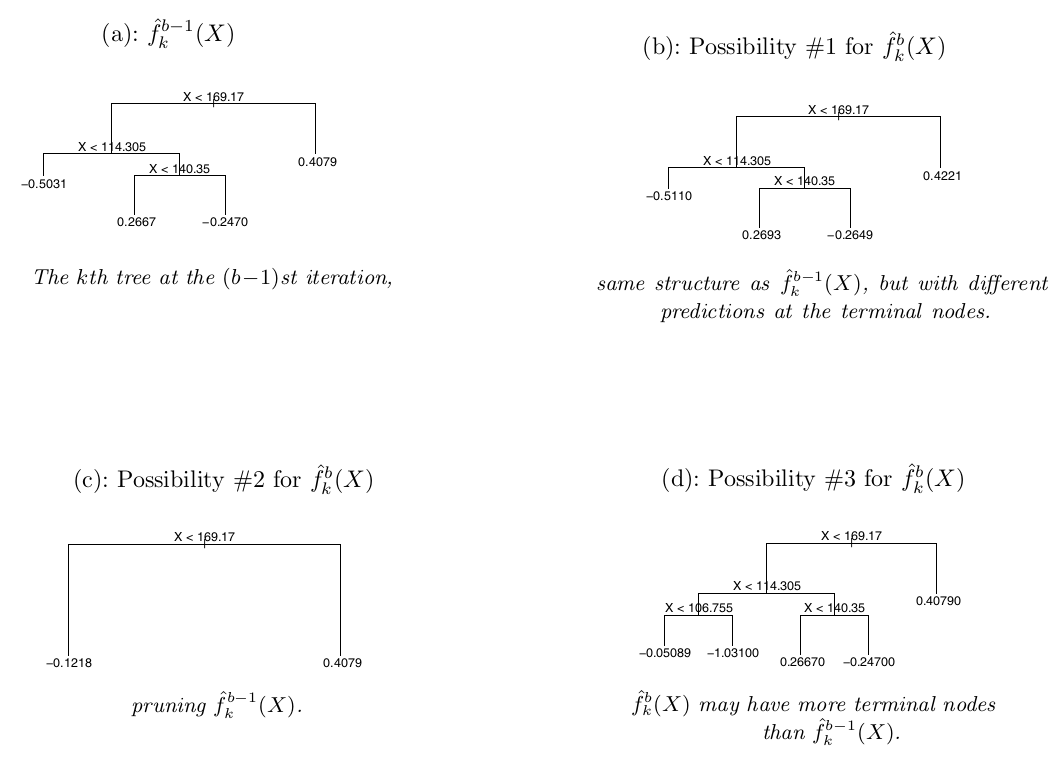
\includegraphics[height=7cm]{bagging-boosting/barts-random.png}
    
\end{figure}
    
\end{frame}